\Grade{高一}
\Name{1v2}\FirstTime{20181111}\CurrentTime{20181117}
% \Name{马灿威}\FirstTime{20181111}\CurrentTime{20181111}
\Topic{任意角、弧度制与三角函数}
\Teach{任意角的三角函数}
\makefront
\vspace{-1.5em}

\section{任意角}
\subsection{角的概念与表示}
{\bf 角的静态定义}::具有公共端点的两条射线组成的图形叫做角。这个公共端点叫做角的顶点,这两条射线叫做角的两条边.\\
\begin{figure}[htbp]
  \centering
  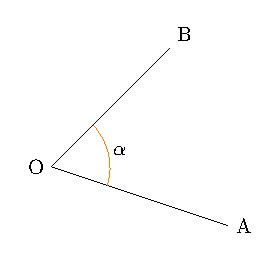
\includegraphics[scale=0.8]{Fig.ArbitraryAngle.pdf}
\end{figure}\par
{\bf 角的符号表示}:上图所示的角可记为“角AOB”、“$\angle{AOB}$”或“$\angle O$”、“角$\alpha$”或“$\angle\alpha$”
“$\alpha$”.\\
三个特殊角:{\bf\kaishu 零角,平角,直角}\par
{\heiti 【思考】}:角的概念是怎么产生的?我们生活中在什么时候用到过角的概念?\par
\vspace{5em}
{角的应用}:\textcircled{1}标记状态;\textcircled{2}标记位置;\textcircled{3}标记过程.\par
{\bf 角的动态定义}:{\bf \kaishu 角}可以看成平面内一条射线绕着端点从一个位置旋转到另一个位置所成的图形.其中,起始位置所在的射线称为{\bf \kaishu 始边},终止位置所在的射线称为{\bf\kaishu 终边}。始边旋转时经过的区域称为{\bf \kaishu 角的内部}\\
特殊角:{\bf\kaishu 周角}\par

{终边相同的角}所有与角$\alpha$终边相同的角,连同角$\alpha$在内,可构成一个集合
$S=\{\beta|\beta=\alpha+k\cdot 360^\circ,k\in\mathbb{Z}\}$.%S={β|β=α+k·360°,k∈Z},
即任一与角$\alpha$终边相同的角,都可以表示成角$\alpha$与整数个周角的和.
\par
{角的(直角)坐标系表示,象限角}
在直角坐标系内,使角的顶点与原点重合,角的始边与$x$轴的非负半轴重合.则依据终边的位置可将角分为:\\
{\kaishu 象限角}:终边在第几象限就第几象限角;\\
{\kaishu 轴线角}:终边落在坐标轴上的角.\\

\section{角的度量,弧度制}
{\bf 角的比较与度量}:角的大小决定于角的两条边张开的程度,张开的越大,角就越大,相反,张开的越小,角则越小。\\
{角的相等}
{角的倍数}
{角的加法}将$\angel 2$的始边与$\angel 1$的终边重合,则始边为$\angel 1$的始边,终边为$\angel 2$的终边的角称为$\angel 1$与$\angel 2$的和\\
{角的减法}将$\angel 2$的始边与$\angel 1$的终边重合,则始边为$\angel 1$的始边,终边为$\angel 2$的终边的角称为$\angel 1$与$\angel 2$的和\\
{角度制}
{思考}角度制下,怎么求角的大小?弧度制下呢?

\startexercise
\begin{exercise}
\item
下列说法正确的是\xz
\xx{终边相同的角一定相等}
{钝角一定是第二象限角}
{第一象限角一定不是负角}
{小于90\textdegree 的角都是锐角}
\begin{answer}B\end{answer}




\end{exercise}
\stopexercise

\section{任意角的三角函数}
\subsection{三角函数定义}
\subsection{同角三角函数的基本关系}
\subsection{三角函数的诱导公式}



\section{课后作业}
